\documentclass[nofootinbib,aps,pre,twocolumn,superscriptaddress,showkeys,showpacs]{revtex4-1}
\usepackage[capitalize]{cleveref}
\usepackage{amsmath, amsthm, amssymb}
\usepackage[toc,page]{appendix} 
\usepackage{graphicx}
\usepackage{subfigure}
\usepackage{wrapfig}
\usepackage{color}
\usepackage{lipsum}% http://ctan.org/pkg/lipsum
\usepackage{graphicx}% http://ctan.org/pkg/graphicx
\begin{document}

\title{Catchy Title Goes Here}
\author{Laura Sampson}
\affiliation{Center for Infectious Disease Dynamics, Pennsylvania State University, State College, PA, 16801}
\author{Matthew Ferrari}
\affiliation{Center for Infectious Disease Dynamics, Pennsylvania State University, State College, PA, 16801}

\begin{abstract}


\end{abstract}
\maketitle

\section{Introduction \label{sec:Intro}}
- Quantifying the size and age distribution of the population susceptible to measles is a critical tool in evaluating vaccination programs and developing interventions.  
- Unfortunately, direct observation of the susceptible population is challenging as it requires a sero-survey which can be cost-prohibitive.
- Previous efforts have estimated the susceptible distribution though demographic models that account for inputs through births and immunization via both vaccination an natural infection.
	- Winter et al (new paper on Madagascar)
	- Merler and the Italian group (http://www.thelancet.com/pdfs/journals/laninf/PIIS1473-3099(17)30421-8.pdf)
- The contribution of natural infection to population immunity can be challenging to estimate. In particular, the age-specific force of infection is not directly estimable from aggregate population time series ? (both papers referenced above rely on SIR models that assume a specific age-structured mixing) 

- The catalytic model has previously been used to estimate the age-specific force of infection from both serological surveys and the cross-sectional age-distribution of measles cases.  The catalytic model, fit to the cross-sectional age distribution of cases necessarily returns an estimate of the age distribution of susceptibles as a by-product.  This suggests that routine case surveillance could be used to generate an estimate of the age distribution of susceptibles.  

- Competing rates ? 
In the vaccine era, however, the age distribution of susceptibility is generated by the sum of the rates of vaccination and natural infection. 

Original applications of the catalytic model assumed that natural infection was the only source of immunity.  

Subsequent analyses have made simple assumptions about the role of vaccination, in particular that the delivery of vaccination is timely, and thus affects the age distribution of the susceptible population only by reducing the force of natural infection.  However, recent work has highlighted significant variability both in the maximum vaccination coverage achieved and the timeliness of vaccination ? that is, the proportion of children receiving vaccination after the recommended age.  Thus, failing to account for the age-specific pattern of vaccination may lead to a biased interpretation of case-data, as children who might be vaccinated later than the recommended age remain susceptible may contribute to incident cases. 

Further, vaccination does not necessarily imply immunization.  The efficacy of measles vaccine is often assumed to be ... (see Uzicanin article) though is also known to improve with age as older children are more likely to have lost maternally transferred antibodies (se many). The effectiveness of vaccine delivered in field settings may also vary dramatically due to stability and effectiveness of the vaccine cold chain.  A comparison of the age-distribution of vaccination and sero-prevalence may highlight areas with low effectiveness, and absent a sero-survey this assessment could be made using age-specific case records.  

Lay out the DRC case study?

Here we present a novel formulation of the catalytic model to estimate the age-specific sero-prevalence, and also the age-specific rates of vaccination and force of infection, and vaccine effectiveness using age-specific vaccine coverage data and case-records. We illustrate performance of this model using both simulated data, and measles case surveillance data from DRC combined with vaccination coverage surveys conducted as part of the 2013-14 DHS.  A contemporary measles sero-survey conducted during the 2013-14 DHS allows us to validate the performance of our estimates of sero-prevelence against direct measurements. We finally present a fit of the model to the surveillance data, vaccine coverage data, and sero-survey and discuss opportunities for combining data sources ? 


\section{Methods \label{sec:Methods}}
\subsection{Competing Rates Model \label{subsec:CompetingRates}}
The classic catalytic model for disease infection, developed in the late 1950's, gives the probability of immunity at age $a$ as
\begin{equation}
p(\mathrm{immune}|a) = 1 - \exp\left(-\int_0^a f(a') da'\right),
\label{eq:CatMod}
\end{equation}
where $f(a)$ is the \emph{force of infection} at age $a$, which can be thought of as the rate of infection at a particular age. This expression is valid in the absence of vaccination, as in this case infection is the only source of immunity. In the case of measles, this expression gives the probability of an individual at age $a$ being seropositive for measles.

In situations in which vaccination is present, vaccination provides a second means of acquiring immunity - the `force of vaccination,' or `vaccination hazard' (vh). If we represent this as $v(a)$, then we can extend Eq.~\ref{eq:CatMod} to give the probability of an individual testing seropositive at age $a$ as
\begin{align}
p(\mathrm{immune}|a)  &= 1 - \exp\left( - \int_0^a f(a') + v(a') da'\right) \nonumber \\ 
&=1 - \exp\left(-\int_0^a f(a') - \int_0^a v(a') da'\right).
\label{eq:CatModSum}
\end{align}

The functional forms of $f(a)$ and $v(a)$ are free to be specified. In this study, we choose to use un-normalized Weibull distributions to parameterize both of these functions, as they have been shown to be sufficiently flexible to match a range of possible forces of infection and vaccination hazards. Thus $f(a) \rightarrow f(a|\mathbb{\psi})$ and $v(a) \rightarrow v(a|\mathbb{\theta})$, where $\mathbb{\psi}$ and $\mathbb{\theta}$ are vectors of the parameters we use for the Weibull distribution - height ($\eta$), scale ($\alpha$), and shape ($\beta$). This gives six parameters that fully specify the forms of $f(a)$ and $v(a)$ from Eq.~\ref{eq:CatModSum} - $\alpha$, $\beta$, and $\eta$ for two independent Weibull distributions. To allow for the fact that not all vaccinations produce immunity, we introduce a seventh parameter - the vaccine effectiveness ($\gamma$). This enters the equation as a multiplier on $v(a)$ that ranges between $0.0$ and $1.0$.

Besides the flexibility of the distribution, another appealing aspect of the Weibull as our choice of parameterization is that it can be integrated analytically, as
\begin{equation}
\int_0^a g(a';\eta,\alpha,\beta) = \frac{\beta}{\alpha} \eta \left( 1 - \exp(-(x/\alpha)^\beta) \right).
\end{equation}
We re-absorb the factor of $\beta/\alpha$ on the r.h.s. of this equation into the parameter $\eta$, and have a final expression for the probability of immunity at a particular age
\begin{align}
p(\mathrm{immune}|a) = 1 - \exp\big\{&-\eta_f\left(1-\exp(-(a/\alpha_f)^{\beta_f})\right)  \nonumber \\ 
&-\eta_v \gamma \left(1-\exp(-(a/\alpha_v)^{\beta_v}) \right)  \big\},
\end{align}
which is parameterized by seven total parameters - $\{\eta_f, \alpha_f, \beta_f, \gamma, \eta_v, \alpha_v, \beta_v\}$.

This expression gives the probability of observing a seropositive individual at age $a$, which accounts for one of our three datasets. The other two are vaccination data and case data. Using the function described above for vaccination hazard, the probability of an individual having been vaccinated by age $a$ is given by
\begin{equation}
p(\mathrm{vaccinated}|a) = 1 - \exp \left\{ - \eta_v (1-\exp\left(-(a/\alpha_v)^{\beta_v}\right) \right\}.
\end{equation}
Finally, the probability of an individual being recorded as a case at age $a$ is the force of infection at that age multiplied by the probability that an individual is susceptible at that age. The probability of susceptibility is of course $1 - p(\mathrm{immune}|a)$, and so the probability of observing a case at age $a$ is
\begin{widetext}
\begin{equation}
p(\mathrm{case}|a) = \left\{ 1 - \exp\left[ -\eta_f \left( \frac{\beta_f}{\alpha_f}\right)\left(\frac{a}{\alpha_f}\right)^{\beta_f - 1}\right] \exp\left[ (a/\alpha_f)^{\beta_f}\right] \right\}
\times \left\{ 1-p(\mathrm{immune}|a)\right\}.
\end{equation}
\end{widetext}

The data we work with (described in detail in Sec.~\ref{subsec:Data}) consists of cases as a function of age, serology tests and results as a function of age, and vaccination status as a function of age for a sample of individuals within a particular province. The likelihood for observing this dataset given values for the model parameters as
\begin{align}
\log \mathcal{L} (\mathbf{c}, \mathbf{v_t}, \mathbf{v_o}, \mathbf{s_t},&\mathbf{s_o}|\eta_f, \alpha_f, \beta_f, \gamma, \eta_v, \alpha_v, \beta_v)\nonumber \\ 
& = \sum_aB\left(v_o(a), v_t(a); p(\mathrm{vaccinated}|a)\right) \nonumber \\
&+ \sum_a B\left(s_o(a),s_t(a);p(\mathrm{immune}|a)\right) \nonumber \\
&+ M\left(\mathbf{c};p(\mathrm{case}|a)\right),
\label{eq:loglike}
\end{align}
where $s_t$ is the total number of individuals tested for IgM seropositivity, and $s_o$ is the number of positive tests; and $v_t$ is the number of individuals surveyed about vaccination status, while $v_o$ gives the number who have been vaccinated. $B$ represents a binomial probability, and $M$ represents a multinomial distribution, and the sums are over age classes. As noted, each data point includes the age of the individual in question.

\subsection{MCMC Sampler \label{subsec:MCMC}}
Given our set of model parameters and the definition of the likelihood in Eq.~\ref{eq:loglike}, we can generate samples of the posterior distributions of the model parameters using Markov chain Monte Carlo (MCMC) techniques. We use the \texttt{PTMCMC} sampler package in Python~\cite{PTMCMC}, which incorporates parallel tempering, differential evolution, and proposals along the eigenvectors of the covariance matrix. This sampler is described in detail in ~\cite{Arzoumanian2014}.

We must specify prior distributions on each of our model parameters before running. These are listed in Table~\ref{table:priors}. 
\begin{table}
\begin{center}
\begin{tabular}{ c|c }  
Parameter & Prior \\
 \hline
 $\alpha_v$, $\alpha_f$ & $\Gamma(2,500)$ \\ 
 $\beta_v$, $\beta_f$ &$ \Gamma(2,5)$ \\ 
 $\eta_v$, $\eta_f$&$ \Gamma(2,15)$ \\ 
 $\gamma$ & $\beta(16,5)$ \\
 \hline
\end{tabular}
\caption{Prior distributions for the seven model parameters. $\Gamma(a,b)$ is the gamma distribution with shape $a$ and scale $b$, and $\beta(c,d)$ is the $\beta$ distribution with shape parameters $c$ and $d$. \label{table:priors}}
\end{center}
\end{table}

We run for $70000$ iterations, keeping every $20$th point in order to decrease autocorrelation. At the end of each run, we calculate the number of effective samples via thinning by the autocorrelation length, as
\begin{equation}
N_{eff} = \frac{N}{auto}.
\end{equation}
Both the effective number of samples and the autocorrelation lengths of all chains are shown in Table~\ref{table:autocorr}.

\subsection{Simulated Data\label{subsec:SimData}}
To confirm that we can accurately recover the force of infection and vaccination hazard using the model we have chosen, we generate simulated datasets consisting of age-specified measles case, vaccination, and serology data using a previously developed, age-structured MSIRV (Maternally immune, Susceptible, Infected, Recovered, Vaccinated) model~\cite{Metcalf2012}. We used demographic parameters from UN estimates for the DRC and increased vaccination linearly from 0 to 50\% over the first 30 years of a 50 year simulation. $R_{0}$ (the number of secondary cases resulting from the introduction of a single infected individual) was assumed to be constant at 15 over the entirety of the simulation. The force of infection (foi) was not directly chosen to be a Wiebull function, but is generated using the specified $R_0$ and WAIFW (Who Acquires Infection from Whom) matrix that describes social interactions as estimated via the POLYMOD study~\cite{Mossong2008}. This means that we cannot directly compare the recovered Weibull parameters to injected parameters, but we \emph{can} compare the recovered foi curve to the true values, as well as the recovered vaccination efficacy ($\gamma$) to the true value. 

While the raw MSIRV model output always entails a value for $\gamma$ of 1, we can simulate scenarios in which $\gamma$ is lower by drawing false positive vaccination responses from a binomial distribution with the corresponding probability, and adding these to the vaccination data generated from our simulation. For example, given that our simulation has a maximum vaccination rate of 50\%, we can simulate a $\gamma$ of 0.75 by assuming that, on average, 67\% of individuals in a given age class will report that they have been vaccinated.

After we generated a full time-series of case, vaccination, and serology data, we then downsampled the simulation results by randomly drawing the same number of observations as are present in the empirical data from the DRC.

\subsection{Data \label{subsec:Data}}

\subsection{Comparing Data and Inference \label{subsec:Comp}}
A standard approach for interpreting the results of Bayesian inference would be to inspect the posterior distributions for the model parameters. But the parameters of our model are not, in themselves, particularly interesting - it is the inferred seroprevalence, case distribution, and vaccination probability that we wish to compare with the data. To do this, we generate the posteriors on $\{\eta_f, \alpha_f, \beta_f, \gamma, \eta_v, \alpha_v, \beta_v\}$ as described, and then draw from these posteriors to generate the seroprevalence, case, and vaccination curves as laid out in Sec.~\ref{subsec:CompetingRates}. Because the vaccine efficacy, $\gamma$, is of interest on its own, we also examine the posterior distributions on $\gamma$ in detail.

In order to assess the impact of different types of data (case, serology, and vaccination data) on our inferences, we run the MCMC package described in Sec.~\ref{subsec:MCMC} on the vaccination and case data alone, the serology and case data alone, and all three datasets together. The results of all of these analyses are discussed below.

\section{Results \label{sec:Results}}
\subsection{Simulated Data \label{subsec:SimDat}}
Although we have chosen a flexible functional form to represent the force of infection and vaccination hazards, we know that that the true functions present in nature are unlikely to be precisely matched by Weibull distributions. This will necessarily lead to some level of biases in our inferences. To understand these possible biases, we analyze simulated data with known foi, vh, and $\gamma$ (vaccine efficacy), and examine the results.  

Figure~\ref{fig:foivhsimdata} shows the injected (dashed lines) and recovered (solid (purple or orange) lines) curves for the force of infection and vaccination hazard from simulated data with vaccine efficacy of $\gamma = 0.9$ (orange) and $\gamma = 0.6$ (indigo). The top panel shows the force of infection, and it is very clear from this panel that a Weibull distribution is not a good fit for the true force of infection, which is bimodal.  Because of this, we do not expect to be able to accurately infer the simulation parameters (i.e., $\gamma$). We examine the inferred values for this parameter in Figure~\ref{fig:veffsimdata}.

\begin{figure}
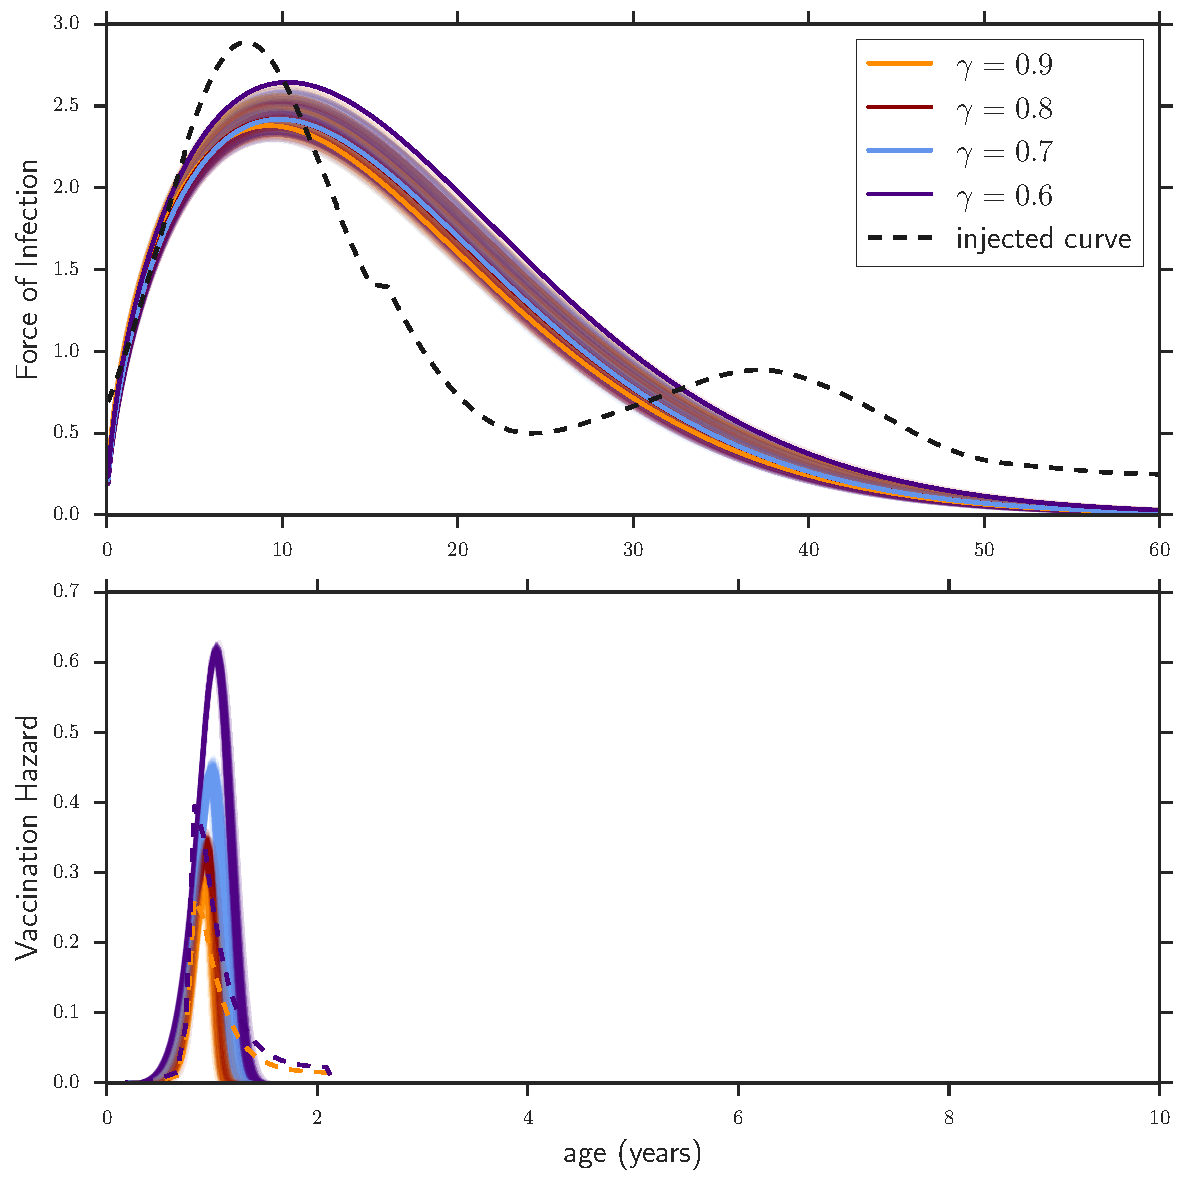
\includegraphics[width=\columnwidth,angle=0]{figures/foivhaz_fakedata_vaxserocase.pdf}
\caption{caption\label{fig:foivhsimdata}}
\end{figure}

\begin{figure}
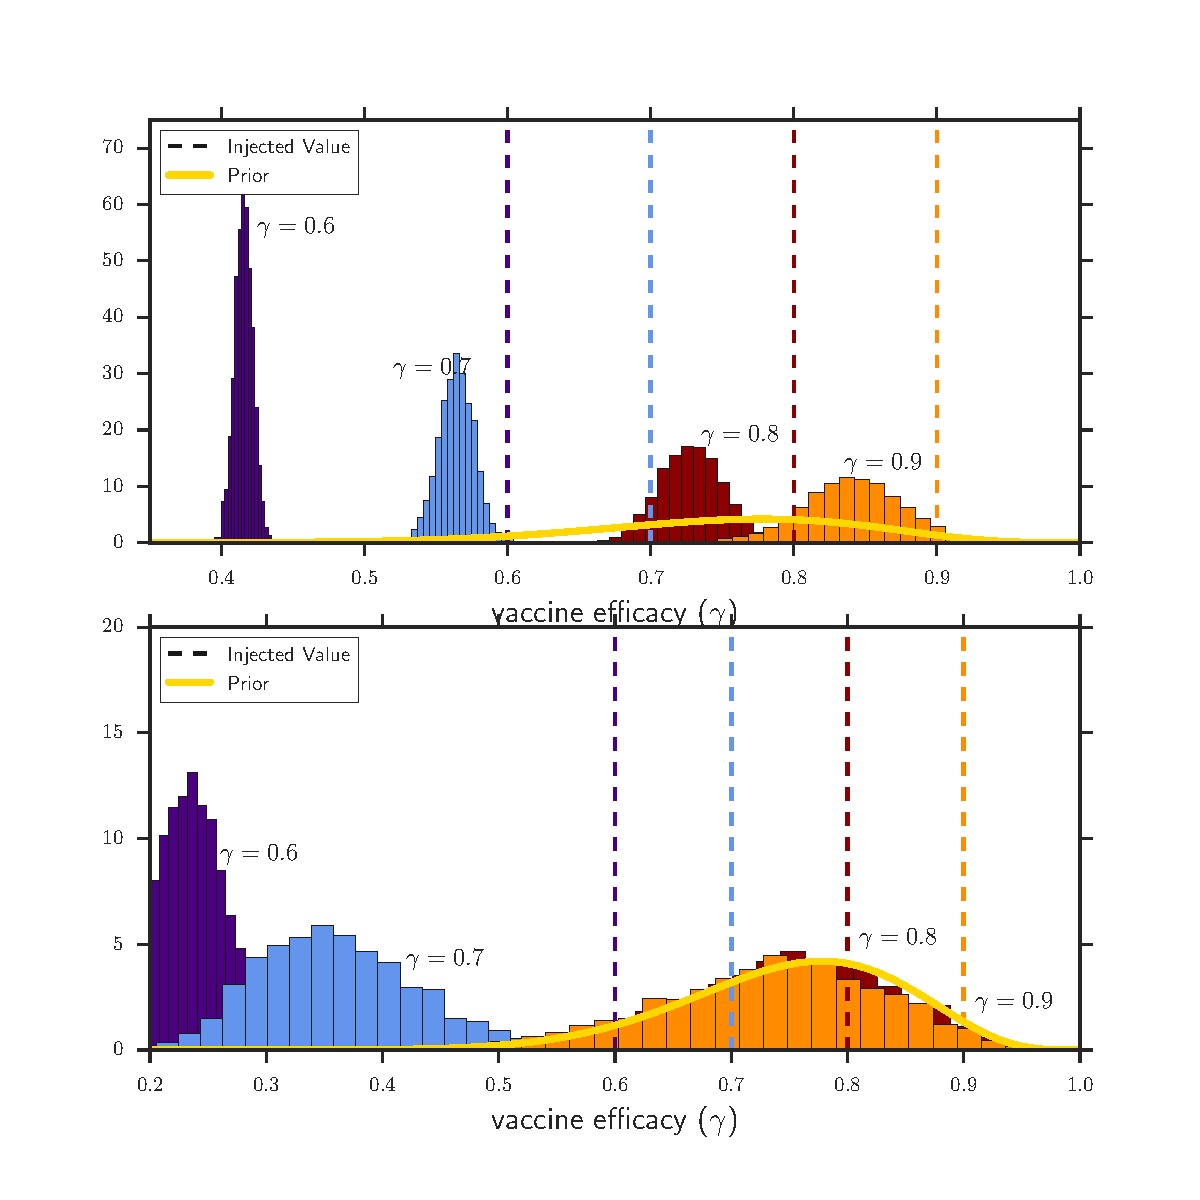
\includegraphics[width=\columnwidth,angle=0]{figures/veff_fakedata.pdf}
\caption{caption\label{fig:veffsimdata}}
\end{figure}

This Figure shows the posterior distributions and injected values for $\gamma$ from simulated datasets with four different values of $\gamma$. The top panel is generated by analyzing all three datasets, and the bottom panel using only case and vaccination data. In addition to the injected values and the posteriors, we also show the prior on $\gamma$ as a yellow line. In the top panel we see, as expected, that the inferred values for $\gamma$ are systematically biased away from the injected values - they turn out to be consistently biased low in this case. Although this means that we do not necessarily infer an accurate value for vaccine efficacy with this data using this model, it is worth nothing that we do infer the correct \emph{ordering} for $\gamma$. That is, if these were four different locations, we would correctly identify the location with the lowest vaccine efficacy.

The bottom panel in this same Figure shows the inferred values for vaccine efficacy using only case and vaccination data - i.e. leaving out the serology data from the analysis. For the higher levels of $\gamma$, the results are dominated by the prior. For the lower values, we are again biased quite low, but also again recover the correct ranking of vaccine efficacy.

Finally, we wish to explore the recovered fits to the true data when analyzing only the case and vaccination data. These results are shown in Fig.~\ref{fig:svcsimdata}. Here, we show the recovered (lines) vaccination prevalence, seroprevalence, and case distribution for simulated data with vaccine efficacy of $\gamma = 0.6$ (indigo) and $\gamma = 0.9$ (orange). The true values for each of these are shown as points. We can see that the case and vaccination data are fit well by the recovered model parameters - unsurprising, given that this is the data that was used in the fitting analysis. The seroprevalence data is also fit well in the case of $\gamma = 0.9$, which recall is one of the values for which the posterior on $\gamma$ is essentially the same as the prior, which includes a lot of weight at the true value. The seroprevalence when $\gamma = 0.6$ is much more biased, although it still follows some of the qualitative features of the true data. Thus for values of vaccine efficacy that are near to the peak of our prior distribution, the seroprevalence inferred using only vaccination and case data is quite accurate. For lower vaccine efficacies, though, seroprevalence data is almost certainly needed to achieve an accurate picture.

\begin{figure}
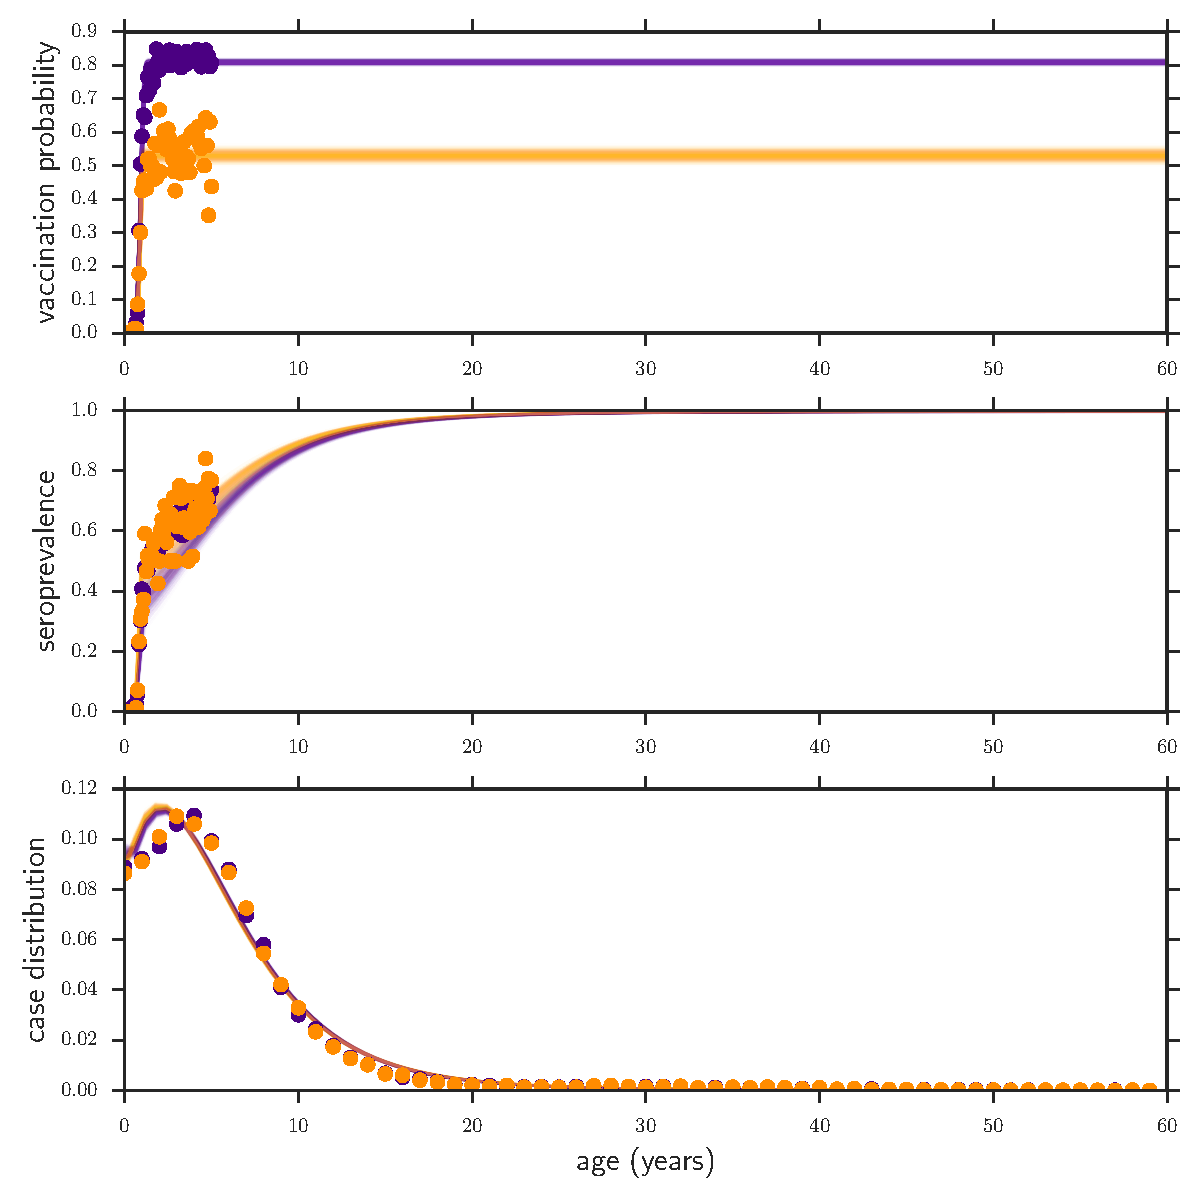
\includegraphics[width=\columnwidth,angle=0]{figures/vsc_simdata_vaxcase.pdf}
\caption{caption\label{fig:svcsimdata}}
\end{figure}

\subsection{DRC Data \label{subsec:DRC}}
Application to the DRC data
	Pairs plots for all provinces ? compare for fits with only case data to fits with case+serology ? discuss any appearance of non-identifiability (?? What is non-identifiability?)	
Figure 2 ? pairs plots for all provinces and two models
	

Figure 3 ? Fitted seroprevalence curves for all provinces (maintain province color scheme throughout all figures). Note that x-scale should be years (up to 20 at least), it doesn?t make much sense over 59m
	- could probably squeeze all 11 into a single figure if played out well

Figure 4 ? fitted hazard functions illustrating variation in vaccination and force of infection.  4-panel, vaccination and FOI hazards for fits with and without serology data. (Note that FOI hazard should be on an x-scale of years, it doesn?t make much sense over 59m)
	- discuss variation observed.  Where is vaccination timely, where is FOI highest

Figure 5 ? comparison of prioritization
	- maybe 2 panels showing the seroprevalence by X years and the estimated vaccine efficacy for case data only v. case plus serology data.

	ASIDE ? would be worth plotting something like maximum vaccination coverage vs. some summary measure of the FOI ? you would expect to see lower FOI in places with higher coverage. If this pattern exists, that would definitely be worth showing!  There might be other summaries of the vaccination hazard that are more informative ? e.g. that account for speed up uptake AND max coverage. 

\section{Discussion \label{sec:Discussion}}
Discussion:

Application for estimating seroprevalence in settings where a sero-survey is not possible 
	? serosurvey may not be feasible to do frequently, but this allows us to use passively collected age-specific case incidence 
	? doing a very wide serosurvey may not be feasible, or practical, but case surveillance lets you see signal across a wide age range

What is the use of this?
	? estimating seroprevalence in the absence of surveys
	? effect size estimate for designing sero-surveys

Discuss the interpretation of the patterns seen in the DRC data 
	? which places have good vaccination, which have high transmission
	? As I recall, some provinces have very wide FOI hazards, indicating that some people are getting infected relatively late in life.  There are lots of possible reasons for this, so should give it some thought.  Could relatively low exposure, so some people are just not exposed until late in life.  Could also reflect inflow of internally displaced people (IDPs).  Speculation depends on the pattern. 

Several things that we haven?t dealt with here, that we?ll need to at least acknowledge:
	- we haven?t dealt with the fact that incidence and vaccination are not stationary
	- we haven?t dealt with supplemental campaigns
	- these are all things that can be dealt with at least theoretically

Take-home message about merging serosurveillance and case-based surveillance

\bibliographystyle{unsrt}
\bibliography{master}

\end{document}







